\section{Evaluation}
\label{sec:evaluation}

Let us now see how well on-demand evaluation works in practice.
We begin by empirically studying the bias and variance of the joint estimator proposed in \refsec{method} and find it is able to correct for pooling bias while significantly reducing variance in comparison with the simple estimator.
We then demonstrate that on-demand evaluation can serve as a practical replacement for the TAC KBP evaluations by piloting a new evaluation service we have developed to evaluate three distinct systems on TAC KBP 2016 document corpus.
%We find that we are able to obtain results of  quality in a cost effective manner.

\begin{figure*}
  \centering
  \begin{subfigure}{0.49\textwidth}
    \centering
    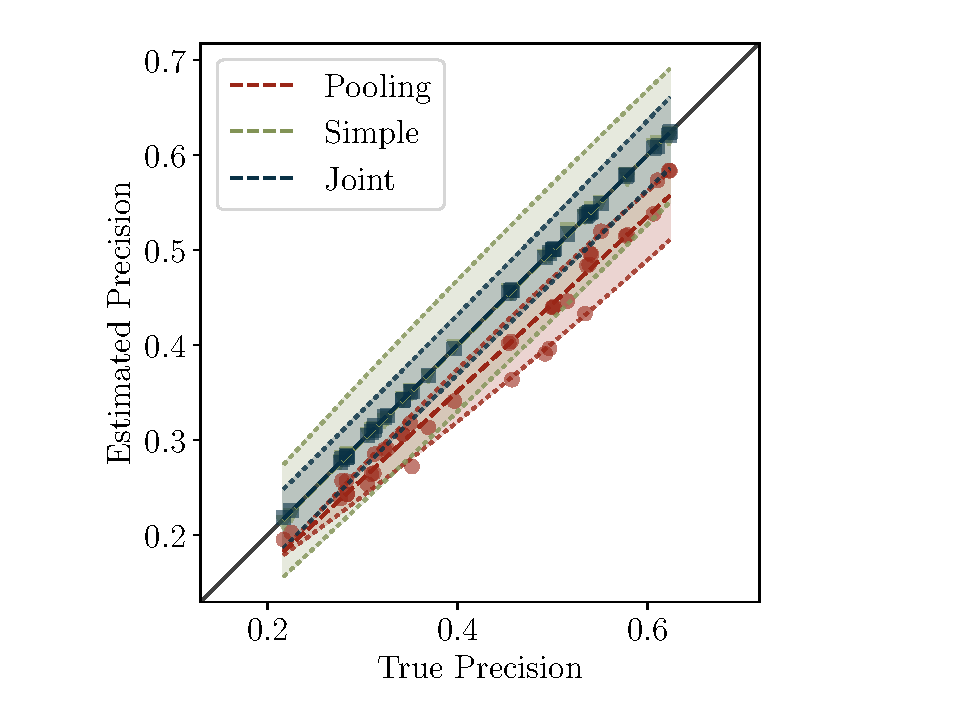
\includegraphics[width=\textwidth]{figures/simulation/simulation-p}
    \caption{}
  \end{subfigure}
  \hfill
  \begin{subfigure}{0.49\textwidth}
    \centering
    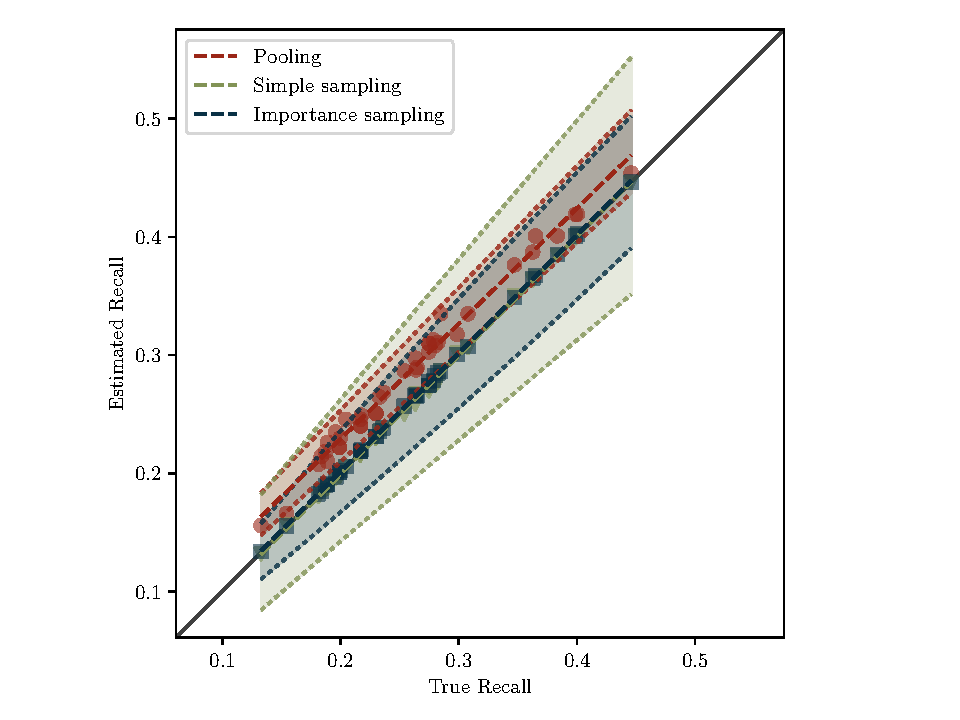
\includegraphics[width=\textwidth]{figures/simulation/simulation-r}
    \caption{}
  \end{subfigure} \\
  \begin{subfigure}{0.49\textwidth}
    \centering
    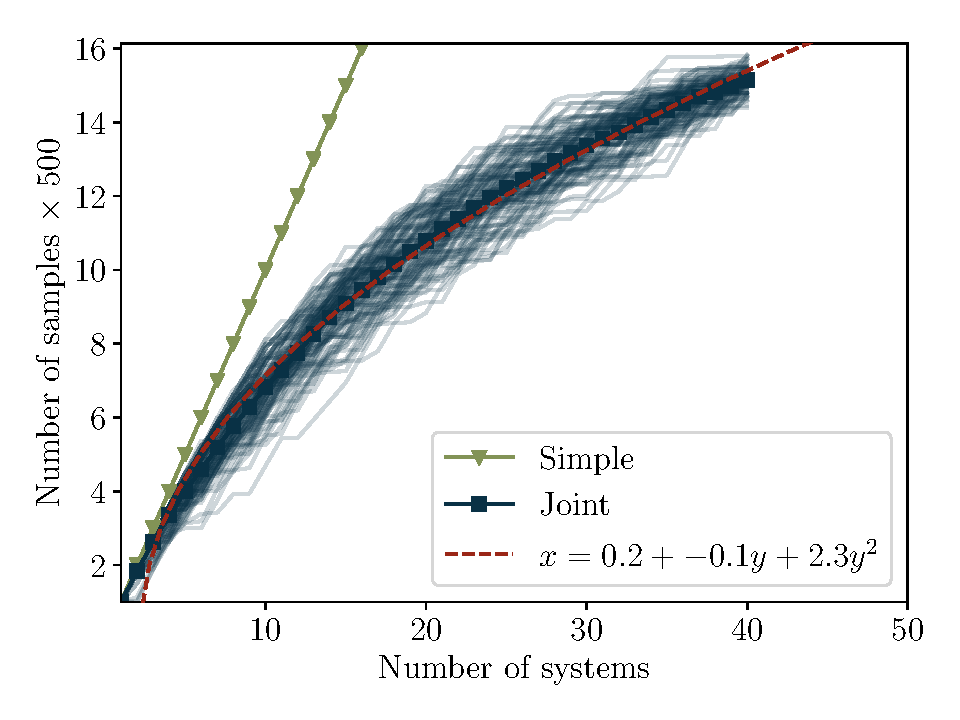
\includegraphics[width=\textwidth]{figures/simulation/simulation-n}
    \caption{}
  \end{subfigure}
  \hfill
  \begin{subfigure}{0.49\textwidth}
    \centering
    \section{Evaluation}
\label{sec:evaluation}

Let us now see how well on-demand open-world evaluation works in practice.
We begin by empirically studying the statistical properties of the proposed estimators by simulating the evaluation procedure on the TAC-KBP 2015 evaluation data and show that the estimators are indeed unbiased and that pooling does reduce variance.
We then show that the on-demand open-world evaluation methodology can serve as a practical replacement for the TAC-KBP competitions by actually running a mock evaluation TAC-KBP 2016 competition using our framework and showing that we obtain results of comparable quality at a fraction of the cost.

\subsection{Studying statistical properties with simulated experiments}
The statistical properties we'd like to study, namely bias and variance, require many repeated trials.
However, because the evaluation data in the TAC-KBP 2015 was collected by completely evaluating all predictions for 317 evaluation entities and 70 systems, we can simulate these trials by imagining that the evaluation data represents the universe of our output and treat a subset of the participating systems as submissions to our framework.

As baselines, we'll compare the precision and recall estimators proposed in \refsec{method} with the pooling-based methodology and with simple precision and recall estimators ($\pih^{(s)}$ and $\rhoh^{(s)}$) that do not reuse samples collected from other systems.
For the pooling-based methodology, we estimate bias and variance over many pool choices.
  On average, each pooled evaluation dataset has about \fake{1,000} evaluated instances.
For the sampling-based methodologies, we estimate bias and variance by running the experiment many times with about \fake{1,000} samples in total from all the different systems, making the two evaluation datasets comparable in terms of how many datapoints are drawn.

In \reffig{statistical-experiment}, we plot the precision and recall estimates made by each of these methods versus their ``true'' values which can be computed by looking at the entire evaluation corpus.
We see from the plots that the pooling-based methodology is significantly biased, while the sampling based estimators are not.
Furthermore, by incorporating samples drawn from other systems, the median variance reduces by a factor of \fake{4.1}, from \fake{0.2} (with the simple estimators) to \fake{0.05} (with the compound estimator).

\subsection{A mock evaluation for TAC-KBP 2016}
In \refsec{application}, we described the necessary elements required to apply on-demand open-world evaluation to KBP.
In particular, we needed to implement two crowd-worker interfaces to verify a relation tuple (i.e.\ evaluate $f(x)$) and to exhaustively annotate a document (i.e.\ to sample from $\sY$).
We have covered the cost and accuracy running these tasks in that section and will now study how well the evaluation framework works end to end. 

Using the algorithm described in \refalg{on-demand-sampling}, we evaluated three distinct relation extraction systems (a rule-based system, a supervised system and a neural network classifier) on 15,000 Newswire documents from 2016 TAC-KBP competition.
Each system uses Stanford CoreNLP~\citep{} to identify entities and the Illinois Wikifier~\citep{} to perform entity linking. 
In total, 100 documents were exhaustively annotated for about \$2,000, and 1000 of each systems submissions were annotated at about \$300 each, with 500 sampled to estimate macro-averaged relation scores and 500 were sampled to estimate macro-averaged entity scores.
\tableref{evaluation-results} presents the results of these systems on the mock evaluation.

\begin{table*}
  \centering
  \begin{tabular}{l l c c c} \toprule
    Scheme      & System    & $P^e (\pm 95\%)$ & $R^e (\pm 95\%)$ & $\fone{}^e (\pm 95\%)$ \\ \midrule
\multirow{3}{*}{Uncombined} &
  Patterns   & \fake{80.4 $\pm$ 3.0}\% & \fake{10.4 $\pm$ 5.0}\% & \fake{18.41 $\pm$ 4.3}\% \\
& Supervised & \fake{60.4 $\pm$ 3.0}\% & \fake{15.4 $\pm$ 5.0}\% & \fake{24.54 $\pm$ 4.3}\% \\
& Neural     & \fake{20.4 $\pm$ 3.0}\% & \fake{30.4 $\pm$ 5.0}\% & \fake{24.41 $\pm$ 4.3}\% \\ \midrule
\multirow{3}{*}{+ Pooling} &
  Patterns   & \fake{80.4 $\pm$ 3.0}\% & \fake{10.4 $\pm$ 3.0}\% & \fake{18.41 $\pm$ 3.0}\% \\
& Supervised & \fake{60.4 $\pm$ 3.0}\% & \fake{15.4 $\pm$ 3.0}\% & \fake{24.54 $\pm$ 3.0}\% \\
& Neural     & \fake{20.4 $\pm$ 2.6}\% & \fake{30.4 $\pm$ 2.7}\% & \fake{24.41 $\pm$ 2.6}\% \\ \bottomrule
  \end{tabular}
  \caption{\label{tbl:evaluation-results} Results from a mock evaluation.}
\end{table*}

%\footnote{A summary of mention-level scores \fake{can be found in the appendix}.}  
% How does cost compare?
% How do absolute scores compare?
Two immediate takeaways are that the precisions of these systems are \fake{on par with} the precisions reported as part of the official 2016 evaluation but the 95\% confidence interval is \fake{almost three times smaller}.
The recall scores on this evaluation are a significantly smaller than on the official 2016 evaluation.
Our explanation for this is that the exhaustive annotation required by our system is far more expansive and finds a lot of new entities that our mention detection systems. \fake{More error analysis.}

    %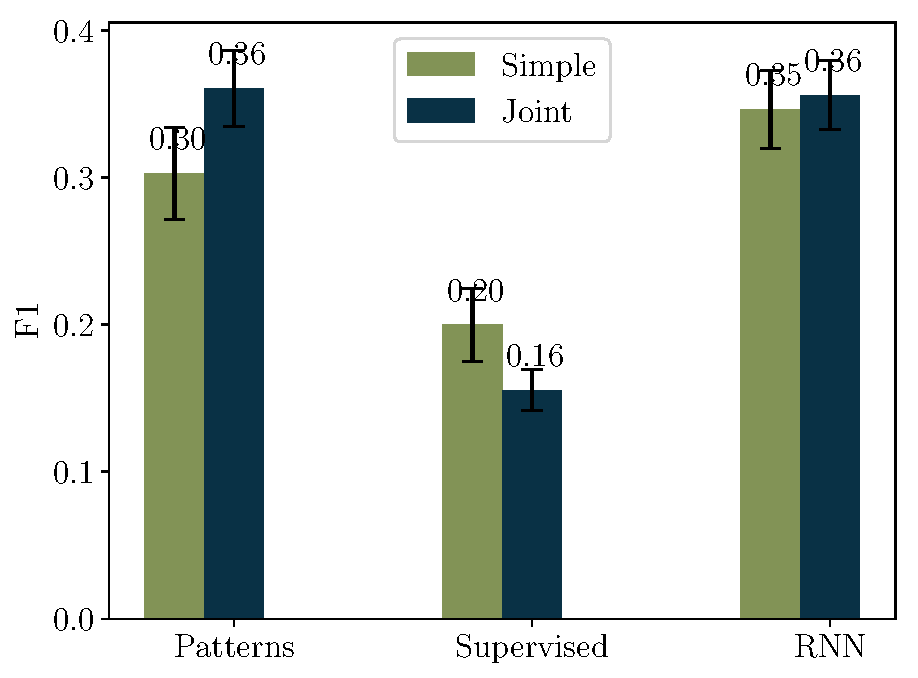
\includegraphics[width=\columnwidth]{figures/kbp2016/kbp2016_f1}
    \vfill
    \caption{\label{fig:evaluation-results}}
  \end{subfigure}

  \caption{\label{fig:simulation}
  \textbf{(a, b):}
  A comparison of estimation error for the pooling, simple and joint estimators on the TAC KBP 2015 challenge.
  Each point in the figure is a mean of 500 repeated trials; dotted lines show the 90\% quartile.
  %The pooling based method uses between 5,000 and 6,000 labeled instances, while the sampling based methods use 
  %approximately 150 samples from each system.
  %Dashed trend lines indicate the mean bias of the estimation method: 
  %Unbiased estimates lie on the $y = x$ line.
  Both the simple and joint estimators are unbiased, and the joint estimator is able to significantly reduce variance.
  \textbf{(c):} 
  A comparison of the number of samples used to estimate scores under the fixed and adaptive sample selection scheme.
  In the simulation, the top 40 systems were evaluated in randomized order to achieve a target variance equal to that obtained with 500 samples for a single system.
  Each faint line shows the number of samples used during a single trial, while solid lines show the mean over 100 trials.
  The dashed line shows a square-root relationship between the number of systems evaluated and the number of samples required.
  \ac{Note: fitting with a cubic gives $x = 0.01 y^3 -0.1y^2 + 1.8 y - 1.1$ with $R=1.0$.}
  Joint estimation combined with adaptive sample selection can reduce the number of labeled annotations required by an order of magnitude.
  \textbf{(d):} 
Precision ($P$), recall ($R$) and \fone{} scores from a pilot run of our evaluation service for ensembles of a rule-based system (R), a logistic classifier (L) and a neural network classifier (N) run on the TAC KBP 2016 document corpus. 
  }
\end{figure*}

\subsection{Bias and variance of the on-demand evaluation.}
Once again, we use all the system predictions from the TAC KBP 2015 evaluation and treat the labeled instances as an exhaustively annotated dataset.
To evaluate the pooling methodology, we contruct an evaluation dataset using
instances found by human annotators and labeled instances pooled from 9
randomly chosen teams (i.e.\ half the total number of participating teams), and
use this dataset to evaluate the remaining 9 teams.
On average, the pooled evaluation dataset contains between 5,000 and 6,000 labeled instances and evaluates 34 different systems (recall that each team may have submitted multiple systems).
Next, we evaluated a set of 9 randomly chosen teams with our proposed simple and joint estimators using a total of 5,000 samples:
about 150 of these samples are drawn from $\sY$, i.e.\ the complete TAC KBP 2015 evaluation data, and roughly another 150 samples from each of the systems being evaluated.

We repeat the above simulated experiment 500 times and compare the estimated precision and recall with their true values in \reffig{simulation}.
The simulations once again highlight that the pooled methodology is biased, while the simple and joint estimators are not.
Furthermore, the joint estimators significantly reduce variance when compared with the simple estimators:
the median 90\% confidence intervals reduce from 0.135 to 0.063 for precision and from 0.141 to 0.081 for recall.

\subsection{Number of samples required by on-demand evaluation.}
Separately, we evaluate the efficacy of the adaptive sample selection method described in \refsec{joint} through another simulated experiment.
In each trial of this experiment, we evaluate the top 40 systems in random order.
As each subsequent system is evaluated, the number of samples to pick from the system is chosen to meet a target variance and added to the current pool of labeled instances.
To make the experiment more interpretable, we choose the target variance to correspond with the estimated variance of having 500 samples.
\reffig{simulation} plots the results of the experiment.
The number of samples required to estimate systems quickly drops off from the benchmark of 500 samples as the pool of labeled instances covers more systems.
This experiment shows that on-demand evaluation using joint estimation can scale up to an order of magnitude more submissions  than a simple estimator for the same cost.

\subsection{A mock evaluation for TAC KBP 2016}
We have implemented the on-demand evaluation framework described here as an evaluation service to which researchers can submit their own system predictions.
As a pilot of the service, we evaluated three relation extraction systems that also participated in the official 2016 TAC KBP competition.
Each system uses Stanford CoreNLP~\citep{manning2014stanford} to identify entities, the Illinois Wikifier~\citep{ratinov2011local} to perform entity linking and a combination of a rule-based system (P), a logistic classifier (L), and a neural network classifier (N) for relation extraction.
%distinct relation extraction systems (a rule-based system, a logistic classifier, and a neural network classifier) on 15,000 Newswire documents from 2016 TAC KBP evaluation.
We used 15,000 Newswire documents from the 2016 TAC KBP evaluation as our document corpus.
In total, 100 documents were exhaustively annotated for about \$2,000 and 500 instances from each system were labeled for about \$150 each.
Evaluating all three system only took about 2 hours. 

%In total, 100 documents were exhaustively annotated for about \$2,000, and 1,000 instances from each system were labeled for about \$300 each, with 500 sampled to estimate macro-averaged relation scores and 500 sampled to estimate macro-averaged entity scores.
\reffig{evaluation-results} reports scores obtained through on-demand evaluation of these systems as well as their corresponding official TAC evaluation scores.
While the relative ordering of systems between the two evaluations is the same, we note that precision and recall as measured through on-demand evaluation are respectively higher and lower than the official scores.
This is to be expected because on-demand evaluation measures precision using each systems output as opposed to an externally defined set of query entities.
Likewise, recall is measured using exhaustive annotations of relations within the corpus instead of annotations from pooled output in the official evaluation.  

%We note that the rule-based system does better on \fone{} because it has significantly higher precision that the other systems, while the RNN system has the highest recall among the three systems.
%We also include TAC KBP evaluation scores for the official submissions that most closely represent these systems.
%The TAC KBP submissions are actually a combination of systems and include filtering and post-processing as required under the evaluation guidelines, e.g.\ submitting a unique instance for each relation.
%While it is hard to directly compare the two evaluation scores, we note that the our evaluation evaluates the rule-based system significantly higher: 
%, which includes submitting a unique instance for each relation, 

\ac{@PL: Should we talk about who pays what on the platform, etc.? A reviewer mentioned this, but I don't think it's appropriate for the paper.}
